\documentclass[../thesis]{subfiles}

\begin{document}

\chapter{Architecture}
Characterization and development of sensor arrays presents a broad
range of research challenges, not least of which relate to data
organization. A \gls{LIMS} adequate to the needs of our example
application must provide a number of interacting software components
to mediate between users and target resources such as data stores,
richly featured research documents, computer-controllable lab
equipment, and collaborators. This chapter abstractly describes the
constituent components of the software framework we have built for
collaborative design, execution, and analysis of experiments. For ease
of reference we refer to our software by its pseudonym ``eGor'', the
Digital Lab Assistant. When describing each element, we document some
of the phases of our iterative design process that led to these
decisions.

\section{Network architecture}
Given that the resources of interest to our software system are
inherently distributed, a careful design of the system's network
interconnect is critical to its scalability, security, and
usefulness. Below we describe the physical system constraints driving
some of our design decisions and explain how we iteratively arrived at
our final design.

\subsection{Physical architecture}
Typical workflows for interdisciplinary digital research involve a
number of computing resources which are physically and logically
separated from each other. These include
\begin{enumerate*}[label=(\roman*)]
  \item{
      individual workstations where researchers perform analysis and
      compose code and documentation,
  }
  \item{
      online information banks such as chemical and biological
      databases,
  }
  \item{
      intranet and cloud storage drives for archiving and sharing
      documents and data,
  }
  \item{
      logs of research-relevant communications such as email
      correspondence, and
  }
  \item{
      dedicated, typically shared scientific resources such as lab
      instruments and high-performance computers.
  }
\end{enumerate*}
In many cases, especially in electrical engineering, a
device we generically categorize as a piece of ``lab equipment'' is a
focus of research in its own right, and can be further decomposed to
include computer controllers, instrumentation electronics, and
physical processes or devices of interest. Often some or all of these
resources interact with each other in an ad-hoc fashion manually
facilitated by users. We believe that tremendous gains can be made for
research organization, accuracy, and reproducibility by coordinating
the interactions between these components with a carefully designed
software framework. A schematic diagram of some of these interacting
components is depicted in Figure \ref{fig:DAQFlow}.

\begin{figure}
  \begin{center}
    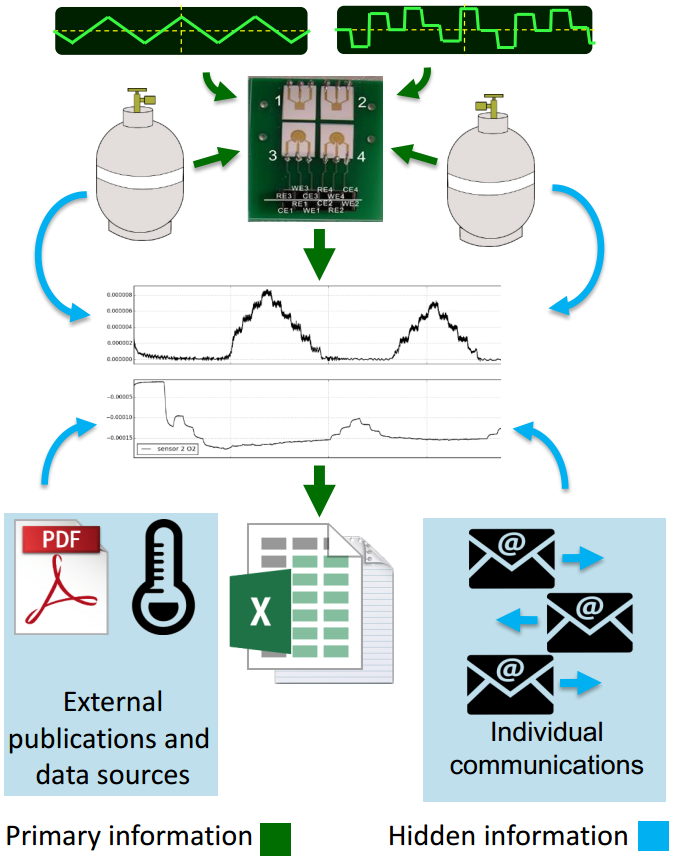
\includegraphics[width=0.8\textwidth]{daq-flow}
  \end{center}
  \caption[Research-relevant artifacts]{
    Representation of some of the digital resources found in
    typical scientific workflows and their relationships. Raw data sets
    captured from an experimental run are often insufficient to
    reconstruct meaningful plots or perform detailed analysis, and
    researchers must rely on undocumented, hidden information sources
    to perform a complete analysis.
    \label{fig:DAQFlow}
  }
\end{figure}

The most important goal of the present work is to automatically
execute physical experiments by employing computer control,
automatically collating raw experimental data with secondary data and
metadata to produce self-contained research artifacts that are more
amenable to unambiguous analysis than present ad-hoc formats.
Ideally we would like for collaborating researchers at different
universities to be able to review each others' experiments in real
time, allowing for continuous feedback between investigators with
different areas of expertise.

Although some pieces of modern lab equipment possess network interfaces
and can directly act as web servers in their own right, a majority of
scientific instruments of interest operate over short-range or legacy
communication links. In order to allow users to remotely interact with
physical resources of this kind, at least one additional machine is
required. This machine is typically represented by a PC physically
located in a research lab and connected directly to external hardware
devices over non-networked connections such as USB.

\subsection{Monolithic approach}
\begin{figure}
  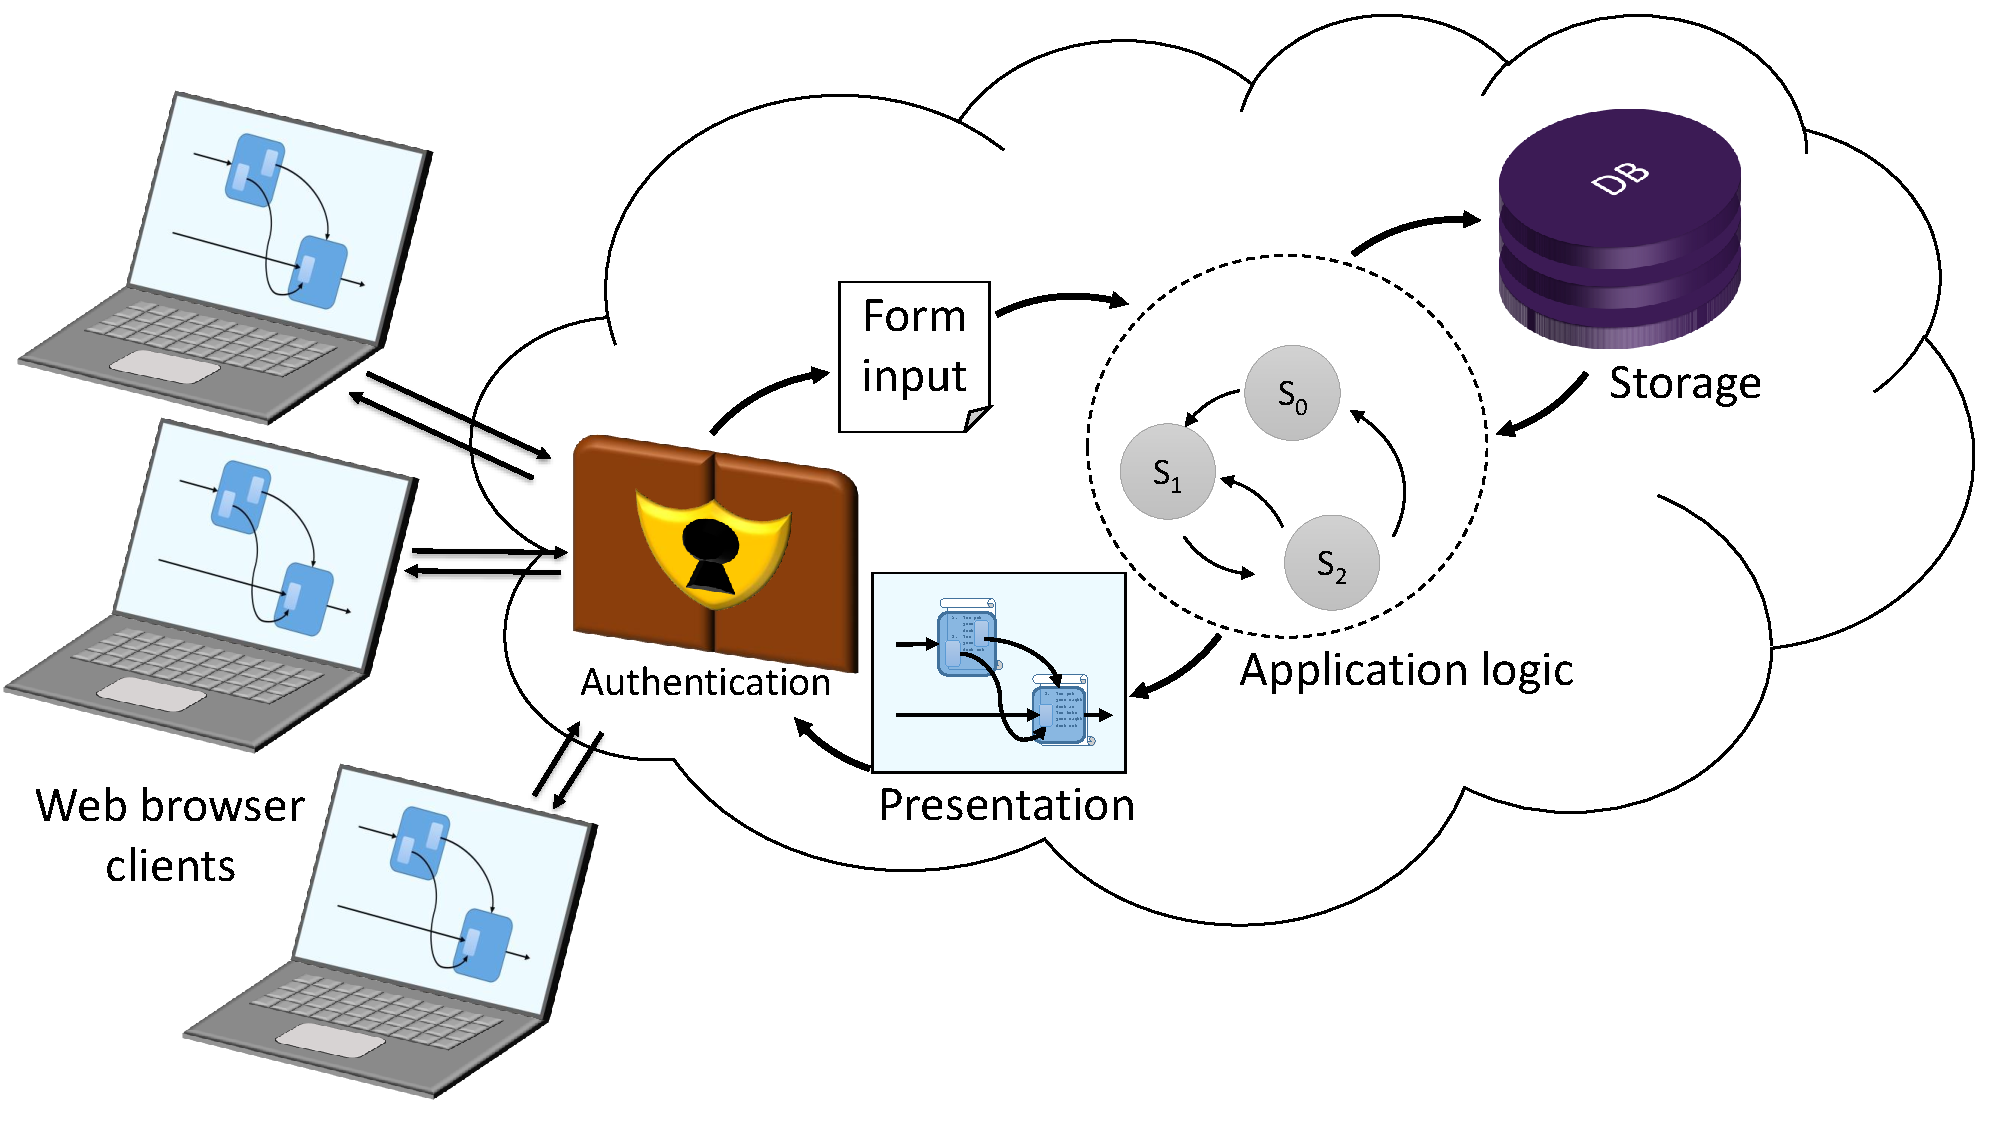
\includegraphics[width=\textwidth]{monolithic}
  \caption[Monolithic web architecture]{
    A traditional ``monolithic'' web application architecture where
    one server process manipulates a database on behalf of many clients.
    \label{fig:Monolithic}
  }
\end{figure}

A traditional architecture for web application software involves a
single server executable serving presentation-layer applications to
clients and making database accesses on their behalf, as in Figure
\ref{fig:Monolithic}. In our case, the server would also mediate
access to lab equipment, providing users with indirect and high-level
access to these resources in much the same way as it abstracts over
the database.

This architecture is attractive for its ease of deployment and its
apparent simplicity, and early in the project's development we pursued
a design along these lines. However, attempting to bundle all of
eGor's server-side functionality into a single program eventually
caused difficulty with system integration. For example, coupling the
code for communicating with lab instruments into the server's
application logic complicates both portions of the program and makes
it difficult to test and develop them in isolation. This agrees with a
common observation \cite{Stephens:2015:BSE:2826034} that architectures
of this kind are often less modular, making them more difficult for
multiple programmers to develop independently and complicating the
process of introducing new functionality. We feel that a more
compartmentalized, modular approach better reflects the structure of
the domain being modeled as well as conferring a number of software
engineering benefits.

\subsection{Microservices}
As opposed to the conventional \gls{frontend}-\gls{backend} divide, some
developers have suggested an architecture for web applications based
on simple communicating modules termed \glspl{microservice}. In a
traditional monolithic architecture, programmers compose a complicated
application hierarchically, using one main module which calls library
functions from many subordinate components.  A microservice
architecture splits functionality into many independent programs which
communicate using ordinary network protocols, and modules are designed
to assume that their dependencies are completely separate programs
potentially running on other machines \cite{Micro14:online}.

This approach promises better modularity than traditional web
applications since capabilities can be added and extended
independently of one another \cite{Balalaie2016}. Since all services
expose their functionality over a similar web \gls{API},
implementations are decoupled from each other and internally have very
different architectures tailored to their special-purpose needs.
Services may even be written in completely different programming
languages. The flexibility that this approach affords is a good fit
with our desire to adapt the framework to meet users' changing
needs. Furthermore, a microservice architecture lends itself naturally
to a design where capabilities and resources are distributed
geographically, as is the case with large, remotely collaborating
groups of researchers. In some cases microservice architectures also
scale better as performance demands on the system increase
\cite{wolff2016microservices}.

\begin{figure}
  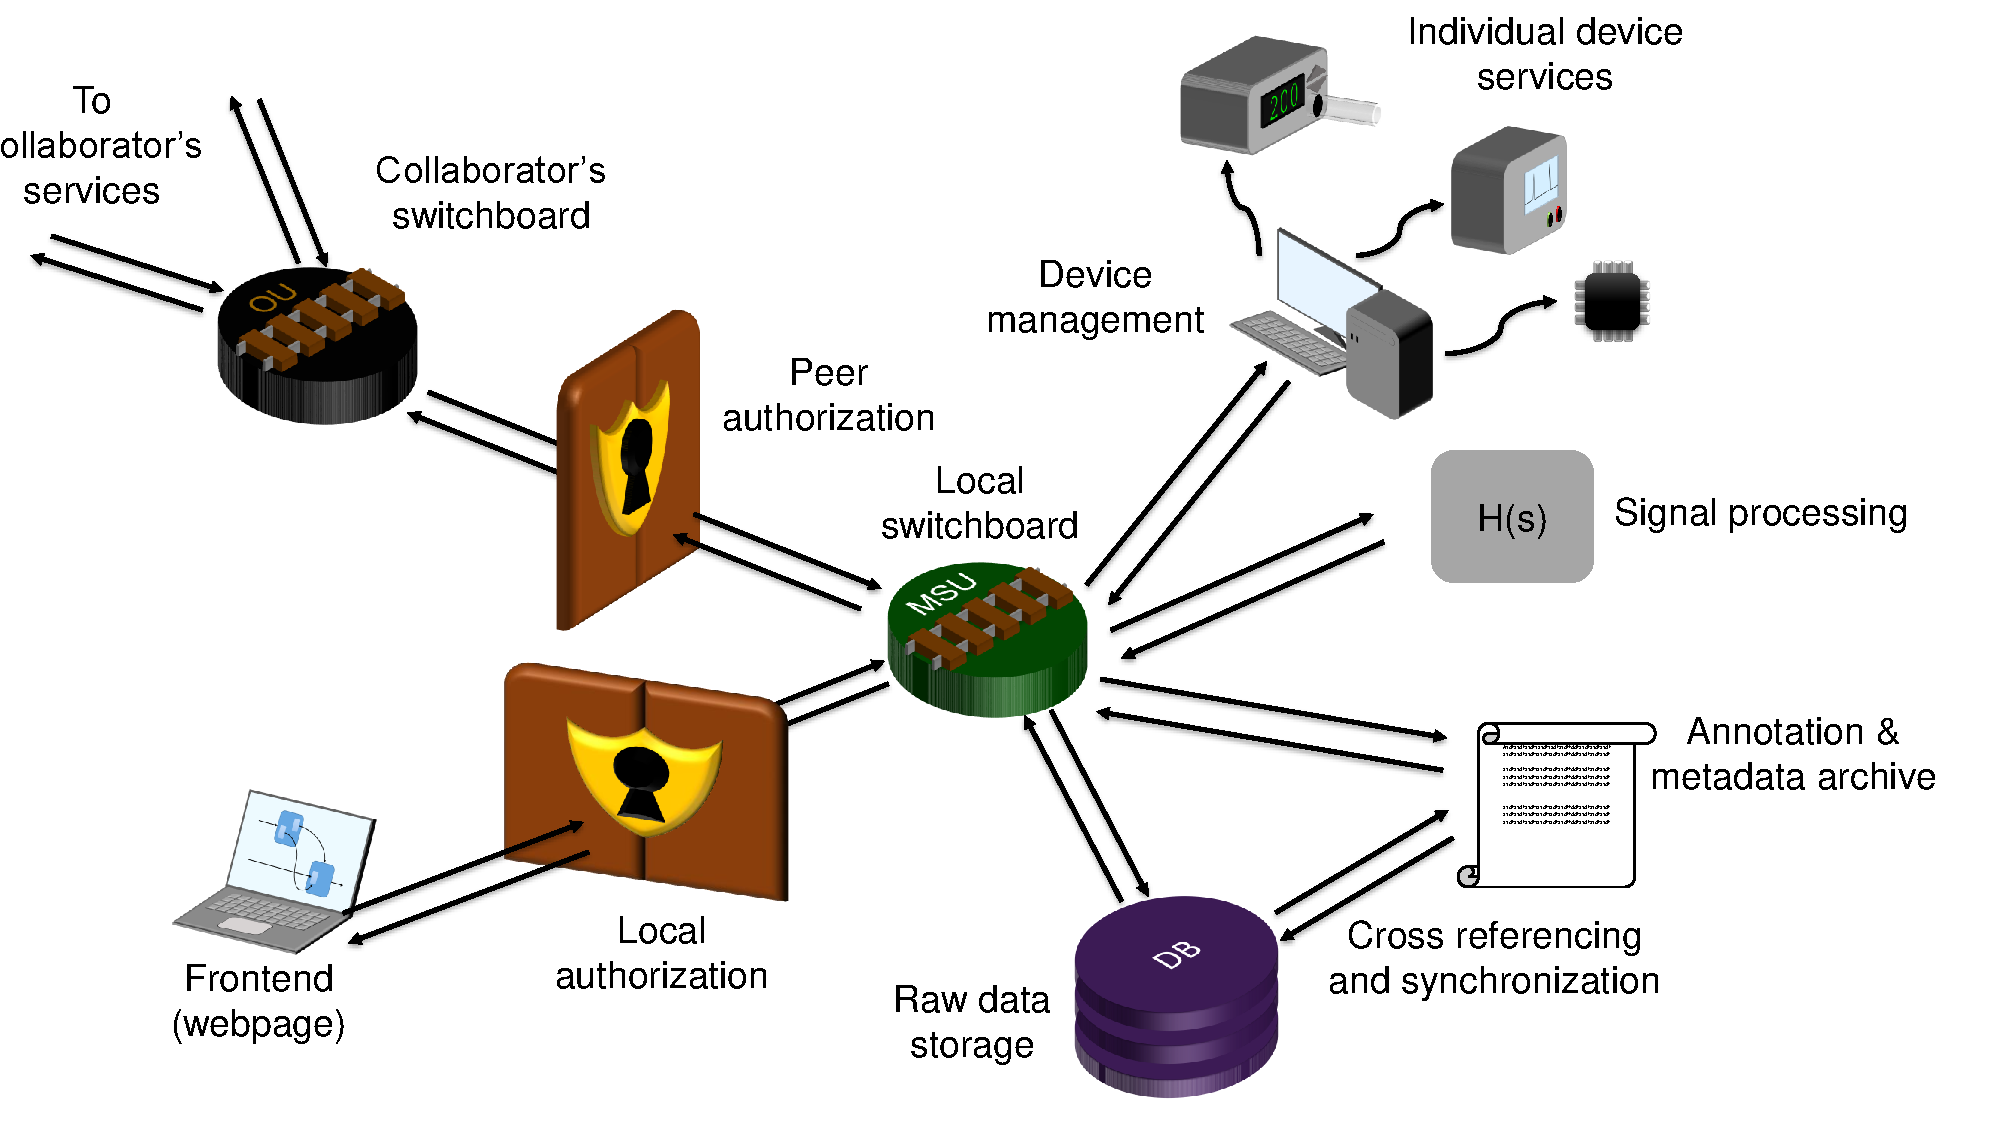
\includegraphics[width=\textwidth]{microservices}
  \caption[Microservice-based web architecture]{
    High-level interconnection between the critical microservices
    composing our final design.
    \label{fig:Microservices}
  }
\end{figure}

A schematic depicting the connections between some of our core
microservices can be found in Figure \ref{fig:Microservices}.
In our approach, no microservice is truly ``central'' -- services may
communicate with any other service provided they know its URI and
present an authorized access token.
Throughout the following, we use the terms microservice and service
interchangeably.

\subsection{Switchboard service}
Despite its internally distributed design, the web application must
present a primary gateway for user interaction. In our design this
role is taken by a microservice we refer to as a \gls{switchboard},
which is primarily responsible for enumerating microservices and
providing proxy access to them at appropriate \glspl{URI}. The
\gls{switchboard} confirms that users are authorized to manipulate their
target resources, then delegates their requests to the microservices
responsible for performing actual resource accesses.

Since the \gls{switchboard} is itself a microservice, multiple \gls{switchboard}
services may be employed by a system, affording system administrators
fine-grained access controls for different components. Additionally,
the \gls{switchboard} of a completely different installation of the software
at a different facility may be treated as an available microservice,
facilitating collaboration by allowing appropriately authorized users
to access external resources as if they were part of one's own
installation.

\section{Device control}
A core goal of our design is to enable researchers to incorporate
choreography of physical lab equipment into the executable workflows
they create. Interacting with the variety of commercial and custom
hardware found in a typical experimental lab requires a flexible
approach, given that computer control interfaces and data formats for
scientific equipment are heterogeneous and very poorly
standardized. This section describes an approach for building a
modular library of device drivers which integrate with the rest of the
eGor framework while providing users with tools for extension and
customization.

\subsection{Instrument manager}
The instrument manager is a service responsible for detecting
connected devices, determining the appropriate device driver for
communicating with them, and presenting a unified interface to the
\gls{switchboard}. This service runs as a background application on
the client machine which is physically connected to lab equipment and
is responsible for relaying control commands to appropriate devices as
well as routing captured instrument data to sinks such as a database
or real-time display viewport. Much as the \gls{switchboard} service
identifies other microservices and mounts them at appropriate
\glspl{URI}, the instrument manager identifies currently connected
devices, determines an appropriate driver and communication protocol
for exchanging messages with them, and exposes their high-level
functionality as an \gls{API} available at an appropriate endpoint,
allowing the rest of the system to behave as if the instruments
themselves were ordinary microservices.

\subsection{Device enumeration}
One of the instrument manager's chief responsibilities is to determine
which devices are presently connected to the PC hosting the
service. The process of establishing a connection with a piece of
equipment and confirming its identity is dependent on the physical
interface as well as device-specific packet formatting. Fortunately,
many scientific instruments follow a standard convention for
identifying themselves to controller PCs. In some cases, however, the
instrument manager must receive explicit user guidance about which
devices are connected.

Once a device produces an identification response or the user
explicitly identifies an attached device, the instrument manager
locates detailed device information by querying our device information
service. In particular, the database record retrieved by the
instrument manager includes a device driver and a protocol stack for
translating low-level device commands to and from a generic high-level
format. This approach allows the device-connected PC to always use the
latest driver for each device, retrieve devices on demand, and
communicate with any device known to a given eGor installation with
minimal user interference. After the downloaded device driver code has
been successfully installed, the instrument manager maps an
appropriate \gls{URI} to the attached device and delegates requests
transmitted to the instrument to the appropriate protocol stack and
device driver.

In earlier iterations of the design, the instrument manager looked for
device drivers and protocol libraries in a directory on its local
filesystem rather than retrieving them from the network. This would
have required users to manually install or update libraries for
interacting with device drivers. Additionally, the database-oriented
approach allows the concrete communication code for a given instrument
to be associated with the abstract data model representing the
instrument as a research artifact, allowing users to examine their
equipment at a finer level of detail when developing an experiment.

\subsection{Device APIs and protocol composition}
The protocol stack bundle associated with a given device is expected
to expose an \gls{API} that allows instruments themselves to be
treated as microservices. The uniformity of this design makes it
possible for the software to model many kinds of remote resources
using a similar approach, and leverages existing network
infrastructure to manage how commands are delegated to devices. An
important responsibility of these device proxy services is translating
complex sequences of commands received by the network to and from
bit-level packets formatted for individual instruments. Borrowing from
Internet design terminology, we refer to the sequence of data
transformations and flow control operations involved in this process
as a \gls{protocolStack}.

To simplify and modularize the creation of communication protocols for
interacting with a wide range of lab equipment, protocol stacks are
designed using a library of basic data transformations as building
blocks. In addition to functionally pure encoding and decoding
processes, a given ``layer'' of a protocol stack may trigger changes
in flow control or provide signals to other layers in response to
certain packets. The resulting framework gives programmers the freedom
to define many different kinds of communication strategies.

By compartmentalizing device drivers in this way, we improve the
maintainability of the instrument management code base and provide
users with the ability to extend eGor with their own
modules. This is especially important for device drivers since the
number of possible communication protocols is far too large to
maintain an adequate library of drivers without community support.



\section{Data model}
eGor must manage data with very heterogeneous structures. In
particular, research artifacts such as equipment, experimental runs,
and publications may be attached to quite different sets of
information. Additionally, we wish to present these records to a
number of services, each of which must have access to enough
information to provide a complex set of functionalities. This section
outlines an object schema focused on flexibility that serves as the
core model for records in our database of research artifacts.
A distinguishing feature of this model is that a given artifact may
have several attached groups of assets including code and data that
indicate how the artifact's attributes should be treated in different
execution contexts.

% A partial \gls{UML} class diagram is shown in figure \ref{fig:DataModel}.

\subsection{Research artifact model}
One of the most basic datatypes in our object model is referred to as
an artifact, and is intended to provide a generic representation of
research-relevant entities such as equipment, experiments,
publications, analysis pipelines, et cetera.  A given artifact is
equipped with a set of ``capabilities'', which are additional data
records that are interpreted in different ways in different software
contexts. Example capabilities a research artifact might have include
a lab notebook's ability to be edited, an experimental workflow's
ability to be executed on physical equipment, an instrument's ability
to operate as a standalone microservice, or an instrument's ability to
capture and tabulate results. Each service may optionally
load some or all capabilities and interpret them in service-dependent
ways to provide extended functionality.

Artifacts may also possess ``assets'', which are files and
resources with internal structures that are opaque to the eGor
system. Examples of assets include images, code for external tools,
and attachments such as PDF documents. Assets are defined by a
\gls{URI} and optional type information and may be accessed or created
on a server's local filesystem by services with appropriate access
permissions. Using an asset rather than an object model to package
data is appropriate when the data does not possess an internal
structure that should be managed by eGor directly. For instance, a
text file containing source code might be an appropriate choice of
asset -- its content may change, but eGor does not need to represent
it internally as a structured object. Managing and interpreting the
content of an asset is typically the purview of external tools, though
operating these tools may be mediated by an eGor service. In the case
of a text file, it would be more appropriate to use existing version
control tools to represent the asset in a structured way.

\subsection{Dataset management}
Ordinarily data are captured via eGor-controlled lab instruments,
adapted via an appropriate protocol stack, and delivered to one or
more data sink services. Typical data sinks include real-time plotting
and signal processing services. To support later analysis and
experiment reuse, one of the core eGor features is a data tabulation
service, which supports streaming live data captures into a data
structure for permanent storage.

To achieve efficient usage of space and fast retrieval times, large
tables of raw data are stored by a different strategy than metadata
documents. To some extent these array data sets can be treated as
ordinary assets belonging to an ``experimental run'' artifact, but
datasets are special because their high-level structure must be
cross-referenced with eGor artifacts encoding their metadata.


Externally generated datasets may also be added to the system by
uploading known file formats, which are dispatched to appropriate
adapter services and committed to the database.  Similarly, previously
recorded datasets may be exported and downloaded for processing with
external scientific computing tools. In these situations, the user is
trusted to provide the structural information needed to enrich and
contextualize the raw data they enter and to appropriately document
the external transformations that take place.



\section{User experience}
Each capability has a corresponding user interface component, allowing
users to manipulate artifacts as well as inspect the system's inner
workings from the graphical browser frontend. Using a similar mechanism to
the approach described above for downloading driver code on demand,
the interface plugin for a given capability is loaded when the
user examines its associated artifact. Artifacts may declare some
capabilities as hidden by default in order to avoid cluttering the
user's workspace.

\begin{figure}
  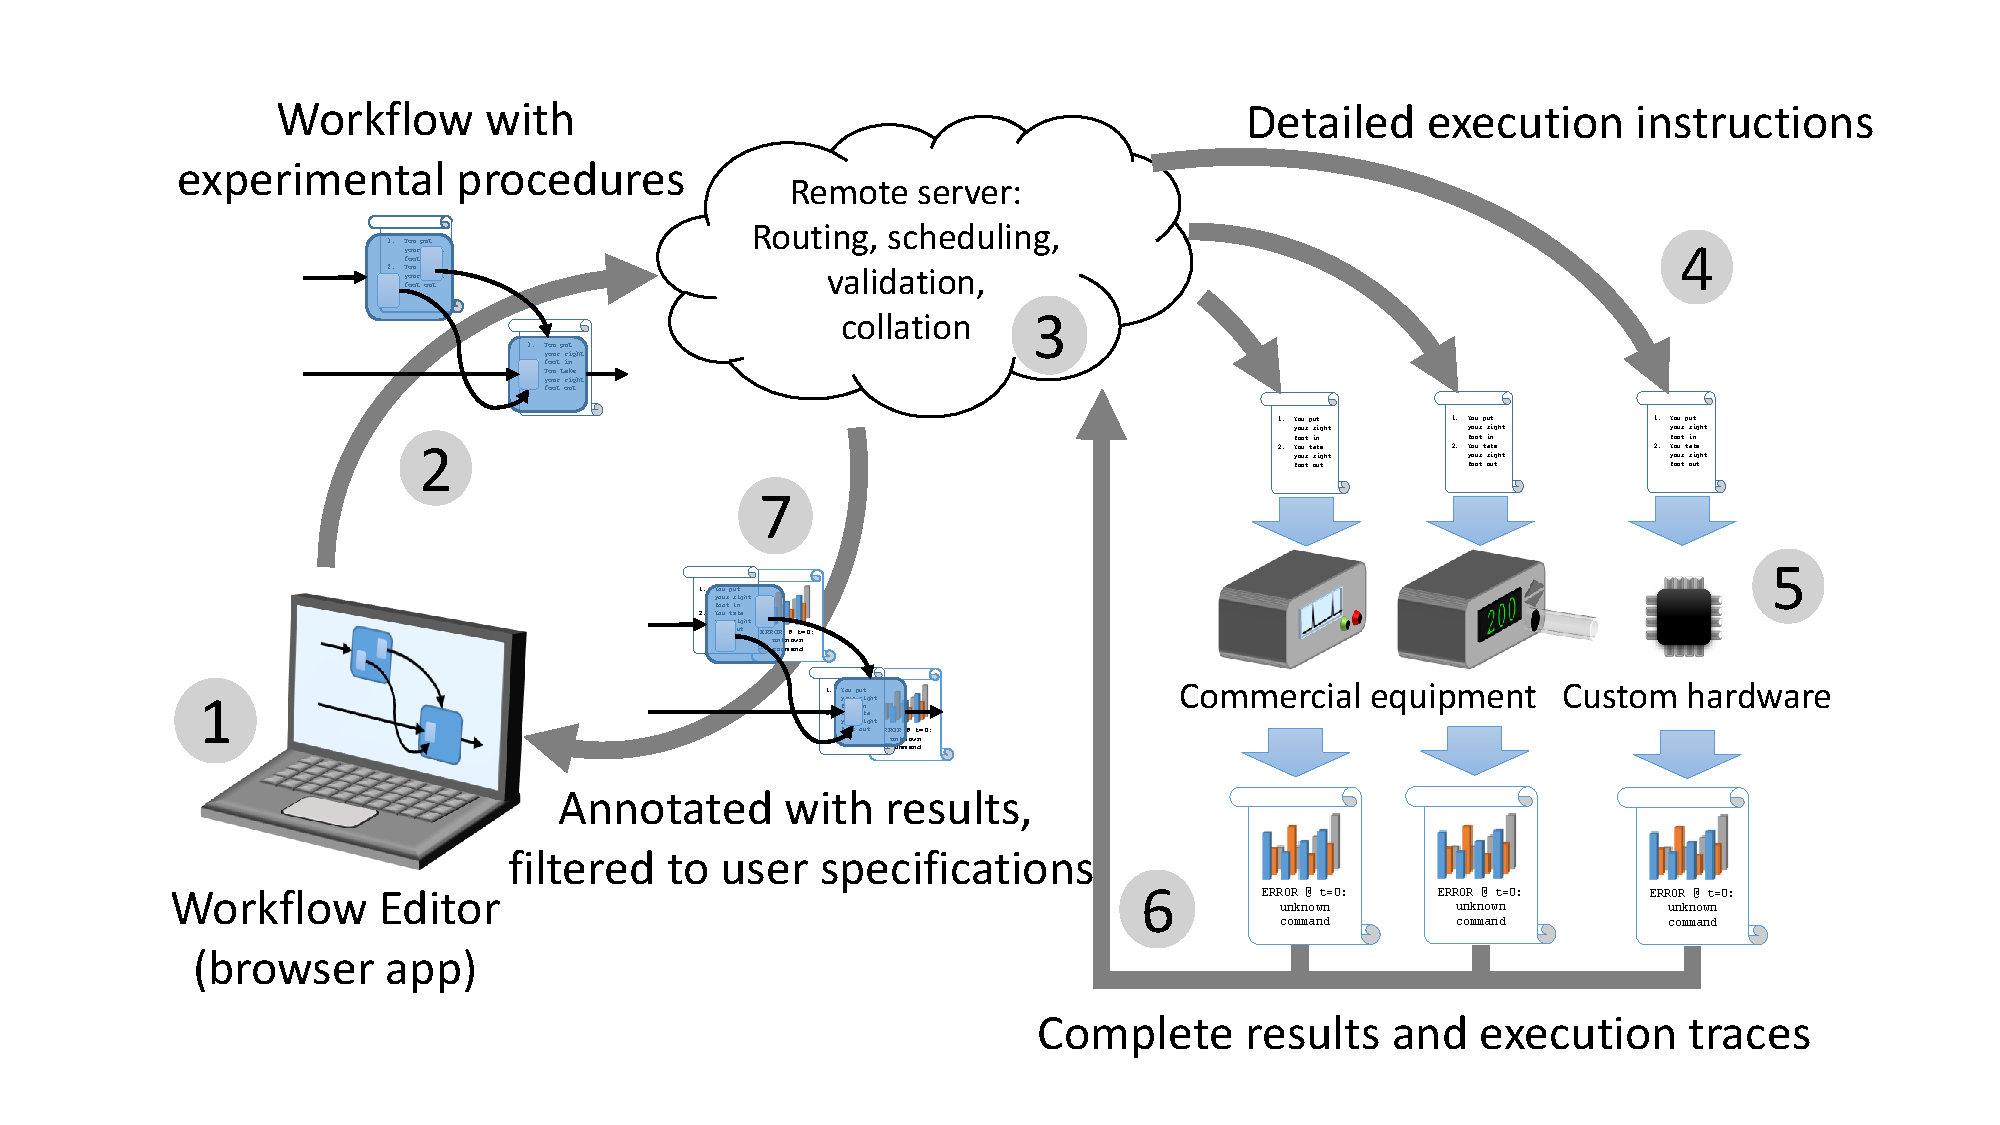
\includegraphics[width=\textwidth]{egor-usage}
  \caption[A typical eGor workflow]{
    A typical sequence of user operations for interacting with eGor to
    design, schedule, execute, and analyze an experiment.
    \label{fig:EgorUsage}
  }
\end{figure}

A usage example of eGor's core functionality from a user's point of
view is depicted in Figure \ref{fig:EgorUsage}, with the following
major phases indicated by numerals in the figure.
\begin{enumerate}
  \item{
      The user constructs a virtual workbench describing the
      configuration and interconnections between their lab
      equipment. The workbench defines the set of resources available
      to one or more workflows, which are specified by wiring
      component inputs and outputs together and providing a script of
      when and how to change parameters as the experiment runs.
  }
  \item{
      The user schedules their workflow to run on the equipment during
      an available timeslot.
  }
  \item{
      The workflow is compiled into a timetable of device-specific
      instructions. Assuming this process completes without errors,
      the workflow is recorded in the database as having been
      scheduled for the desired execution time.
  }
  \item{
      The scheduled, compiled workflow is submitted to the instrument
      manager to await execution. Nearing the scheduled experiment
      time, an experiment executor service ensures that the experiment's
      preconditions are met.
  }
  \item{
      The experiment executor service executes desired hardware
      commands at the user's specified times. As the experiment runs,
      real-time data is captured and streamed to the data sinks
      indicated in the workflow specification, allowing researchers to
      confirm that the experiment is proceeding as expected.
  }
  \item{
      A complete log indicating the status of the experiment, any
      errors, and any failures to meet the user's constraints is
      returned to the server for archiving and later review. The
      experiment executor service attempts to confirm that experimental
      postconditions are met and prepares for the next scheduled
      experiment.
  }
  \item{
      The raw output log is transformed and returned to the user,
      producing a filtered result structure that reflects only the
      user's specified outputs of interest.
  }
\end{enumerate}



\section{Security model}
Especially when dealing with sensitive scientific data and remote
access to expensive lab equipment, careful access control is an
important architectural concern. As in a traditional client-server
model, when clients authenticate themselves to the system they are
provided with an access token that can be used to preserve their
credentials between browser sessions. When a user makes a request
through a sequence of proxy services, this access token is provided
along with the request and is passed along to each service on the way
to the request's destination. Each eGor service requires client
services to produce an access token before it will perform work on
their behalf, and a service may query a user management service with
an access token to determine the identity of a user and whether their
access is authorized.

Switchboard services for collaborator's
installations may also query the user management service of the
installation requesting access in order to either deny access to a
token outright or to generate an access token corresponding to a
foreign user.  Users may provide labmates or collaborators with
authorization rights to services and artifacts which they own or
manage, and doing so modifies the list of user IDs the service will
permit to access certain operations.



\section{Summary}
We have outlined an end-to-end system architecture for a set of
interacting e-laboratory software components. We feel that this
approach provides a reasonable combination of our target system's
ambitious list of desirable features and includes a number of
noteworthy design ideas. In particular, we believe that the emphasis
on modularity from the ground up will be rewarded by benefits in
scalability, extensibility, and user customization that are not seen
in existing \gls{LIMS}. In the next chapter we describe our efforts
to implement this vision in detail.



\end{document}
